\chapter{Description macroscopique du bois et fondements de la physiologie des arbres}

\begin{abstract}
La science du bois est un domaine d'étude consacré principalement à l'utilisation du bois comme matériau. Or, contrairement à la plupart des autres matériaux utilisés dans la vie de tous les jours, le bois est issu d'un organisme vivant. Pour bien comprendre son anatomie, sa structure et, ultimement, l'impact de ceux-ci sur l'utilisation du bois comme matériau, il est fort utile d'avoir une compréhension au moins sommaire du fonctionnement des plantes qui produisent ce matériau. La physiologie végétale, ou plus particulièrement la physiologie de l'arbre, est la discipline qui s'intéresse au fonctionnement des plantes. Ce chapitre présente certains des fondements du fonctionnement des arbres qui sont utiles à la compréhension de l'anatomie du bois. Comme ils sont intimement liés, la description du fonctionnement de l'arbre est complémenté par une description de son anatomie et sa structure à l'échelle macroscopique. L'identification précise du bois se fait au niveau cellulaire, c'est-à-dire au niveau \og microscopique \fg. Par contre, il est possible de reconnaître un certain nombre de caractères du bois à l'œil nu ou avec une lentille de faible grossissement. On parle alors des caractéristiques \og macroscopiques \fg du bois qui constituent des éléments fort utiles à l'identification.
\end{abstract}

\minitoc
 
\section{Plantes ligneuses et non-ligneuses} 

Le bois est un matériau provenant des plantes. Par contre, les plantes ne possèdent pas toutes des tiges ligneuses et celles qui en possèdent une ne produisent pas toutes du bois exploitable à l'échelle industrielle, c'est-à-dire que les espèces ligneuses ne sont pas nécessairement toutes d'importance commerciale. 

\subsection{Critères définissant une plante ligneuse}

\begin{description} 
\item[Une plante vasculaire]est une plante possédant des tissus de transport spécialisés : 
 
\begin{itemize}
\item xylème (bois, présence de lignine) 
\item phloème (écorce interne)
\end{itemize}
 
\item[Une plante vivace]est une plante vivant plusieurs années. 
\item[Une tige persistante]ne meurt pas à chaque année. 
\item[Croissance de la tige en diamètre] une plante ligneuse a une croissance en diamètre due à l'activité d'une couche de cellules en constante division cellulaire appelée cambium. 
\end{description}
 
\subsection{Types de plantes ligneuses} 
 
\begin{description}
\item[Arbres] un arbre fait plus de 7 m de hauteur à maturité sur un sol fertile et possède une tige principale 
\item[Arbustes] un arbuste fait rarement plus de 7 m de hauteur à maturité et est habituellement formé de plus d'une tige. 
\item[Lianes] une liane est une plante ligneuse grimpante.
\end{description}

Il faut noter qu'une plante d'une espèce donnée peut être arbustive à la limite de son aire de distribution et arborescente ailleurs. 
 
\subsection{Les principales parties d'un arbre}
 
Les principales parties d'un arbre sont illustrées à la Figure~\ref{arbre}. On reconnaît le houppier (ou cime vivante), la tige, les racines, le bois d'aubier, le bois de duramen, le cambium, le phloème (ou écorce interne) et l'écorce. 
 
\subsection{Croissance de la tige}\label{croissance_cernes}
 
La structure de la tige est illustrée à la Figure~\ref{croissance}. On remarque qu'à chaque année un cerne annuel s'ajoute, ce cerne formant une structure tridimensionnelle en forme de cône se déposant sur le bois formé au cours de l'année précédente. Il est à remarquer que l'âge obtenu en comptant les cernes annuels dans le plan transversal (RT) diminue de la souche vers le haut de la tige. Il s'agit ici de l'âge cambial, c'est-à-dire de l'âge du cambium à un niveau donné \\
 
La croissance de la tige s'effectue de deux façons. En hauteur par l'action des méristèmes apicaux (méristèmes primaires) et en diamètre par l'action du cambium (méristème secondaire).\\
 
Dans les zones tempérées, on peut distinguer un cerne annuel par année dû à l'arrêt de la croissance à l'automne. Dans les zones tropicales humides, on ne peut distinguer de cernes annuels car la croissance ne s'arrête pas. Des cernes annuels peuvent toutefois se former suite à des périodes de sécheresse. 
 
\subsection{Forme de la tige}
 
La Figure~\ref{types_arbres} présente la forme typique des arbres résineux, des feuillus et des monocotylédones ligneux (bambous et palmiers). On remarque la tige principale des résineux qui s'étend de la souche au sommet du houppier, ce qui les favorise pour la production de pièces de grande longueur pour usage en charpente. 


\begin{figure}[ht]
\centering
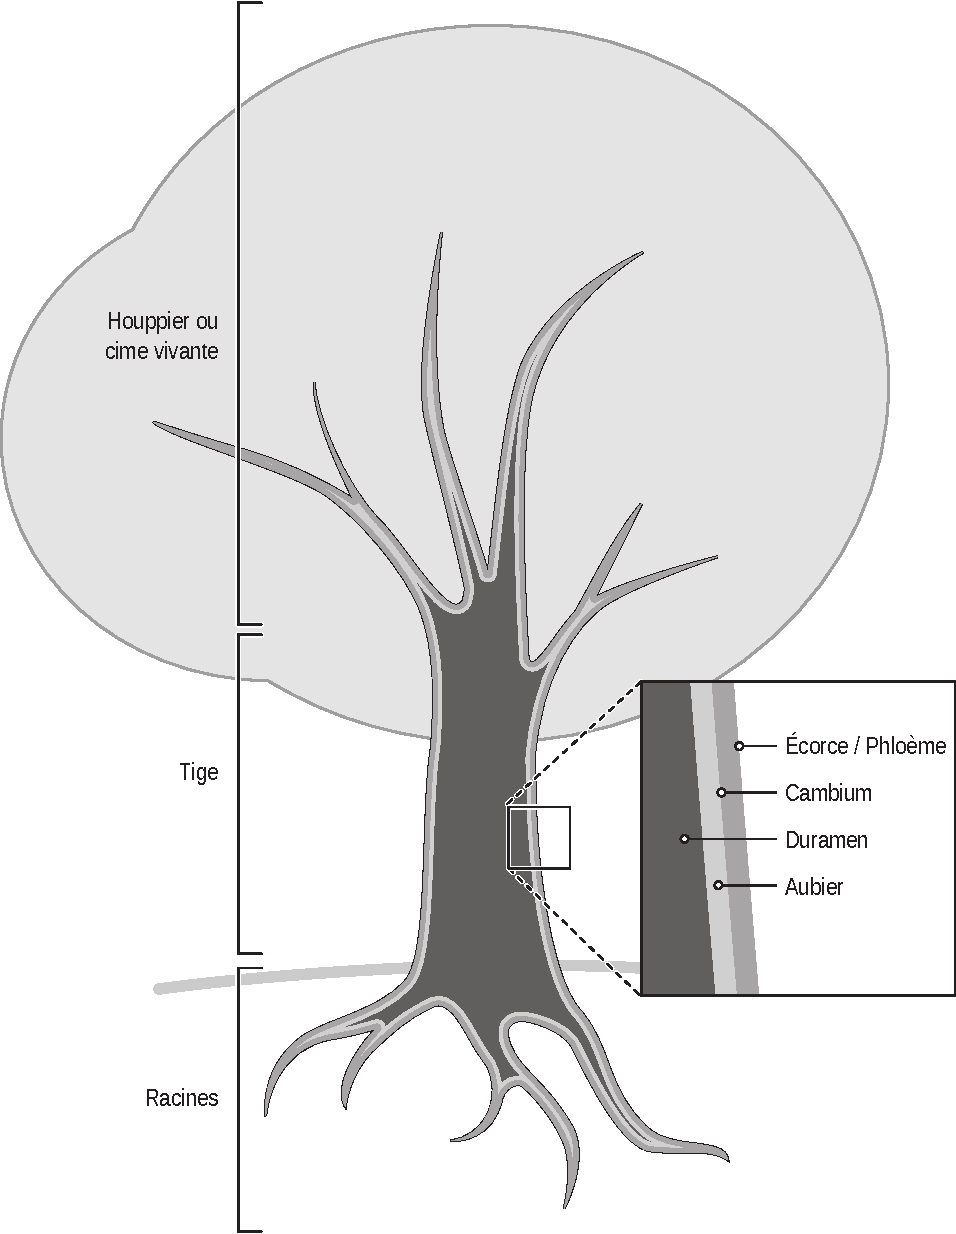
\includegraphics[scale=0.6]{img/ch2_partie_arbre}
\caption{Principales parties de l'arbre et de la tige (adapté de \cite{hoadley1990identifying}). Image préparée par Julie Ferland pour \cite{achim2010dendroecologie}}
\label{arbre}
\end{figure}

\begin{figure}[ht]
\centering
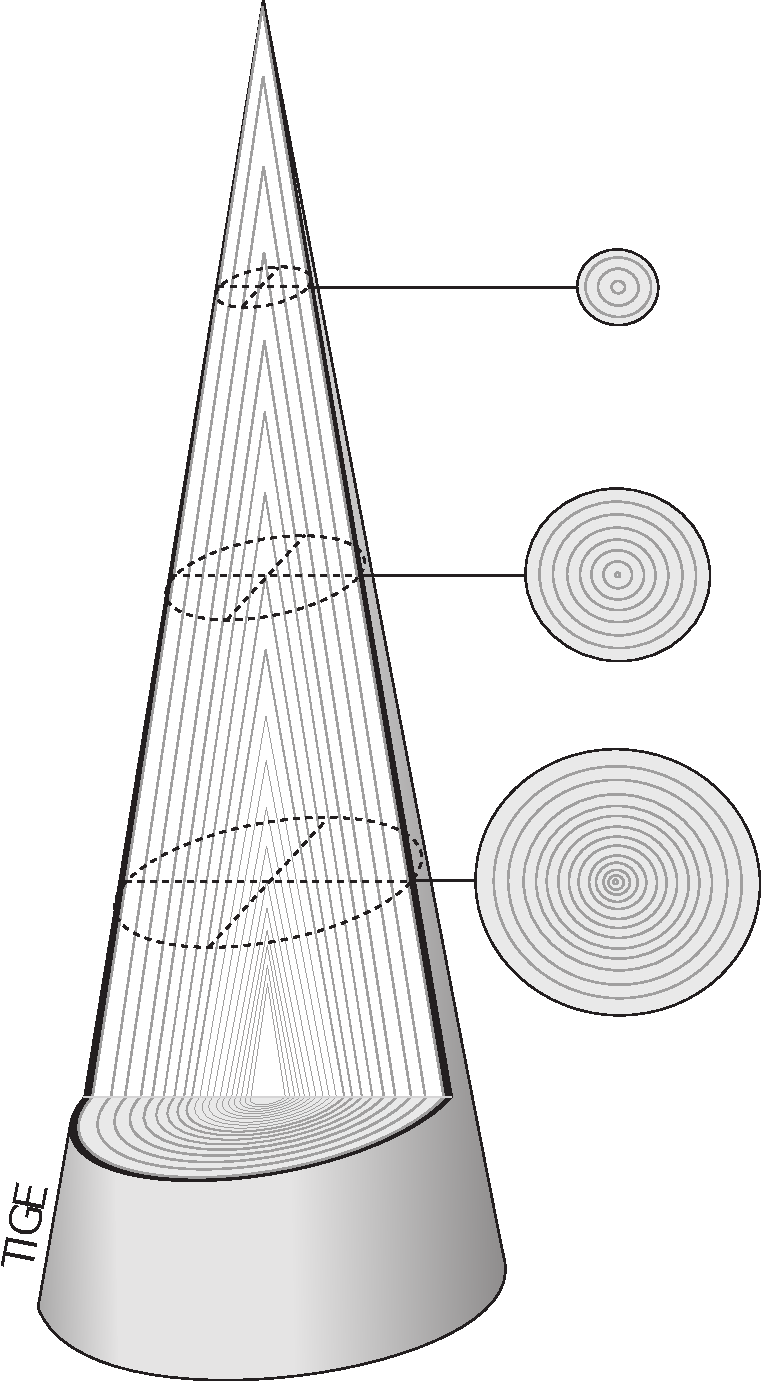
\includegraphics[scale=0.5]{img/ch2_croissance_cernes}
\caption{Représentation de la croissance annuelle de la tige. Image préparée par Julie Ferland pour \cite{achim2010dendroecologie}}
\label{croissance}
\end{figure}

\begin{figure}[ht]
\centering
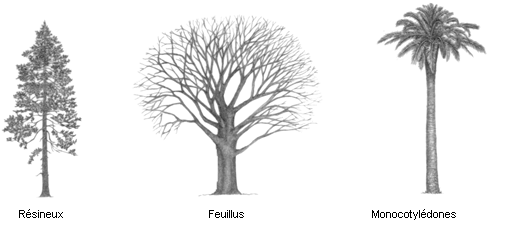
\includegraphics[scale=0.9]{img/ch2_types_arbres}
\caption{Forme typique des arbres résineux (ou conifères), des feuillus et des monocotylédones ligneux (bambous et palmiers) (adapté de \cite{hoadley1990identifying}}
\label{types_arbres}
\end{figure}

\subsection{Facteurs déterminant l'importance commerciale d'un bois}

\begin{description}
\item[Taille des arbres] La transformation des bois tend généralement à être plus rentable lorsque la taille des arbres augmente. 
\item[Qualité du bois pour usage commercial] Résistance mécanique, durabilité, stabilité dimensionnelle, aptitude au façonnage. 
\item[Accessibilité des peuplements] Infrastructure disponible et relief. En forêt tropicale, peu d'infrastructure et des peuplements mixtes. Dans l'est de la Russie, beaucoup de volume résineux disponible mais peu d'infrastructures.
\item[Volumes disponibles] Volume suffisant pour justifier le développement de l'infrastructure et disponibilité d'autres espèces plus intéressantes au niveau technologique 
\item[Connaissances technologiques] Par exemple, dans les années 1980 le peuplier faux-tremble est passé d'une espèce pour laquelle il y avait peu d'usages à une espèce très convoitée aujourd'hui à cause du développement de l'industrie des panneaux de lamelles orientées (Oriented Strandboards, OSB). 
\end{description}

\subsection{Bois résineux et feuillus}
 
Globalement, les bois résineux sont utilisés en volume plus important que les bois feuillus en Amérique du Nord. Par exemple, au Québec en 2005 on a produit \numprint{15556000} m\up{3} de bois de sciage résineux comparativement à \numprint{846600}  m\up{3} de bois feuillus pour un total de \numprint{17402700} m\up{3}. Il y a cependant peu d'espèces commerciales chez les résineux, mais elles occupent une place importante sur le plan économique pour les raisons suivantes : 

\begin{itemize}
\item Les peuplements de résineux sont purs ou comptent peu d'espèces, donc sont faciles à récolter 
\item Les forêts résineuses sont principalement situées dans des pays industrialisés
\item La tige est plutôt droite avec un défilement généralement faible ce qui est approprié pour le bois de construction 
\item Le bois homogène est adapté à la production de masse du bois de construction 
\end{itemize}
 
Les bois de feuillus sont constitués d'un plus grand nombre d'espèces offrant des bois dont les caractéristiques très variées déterminent des usages plus diversifiés. 

\subsection{Volume marchand brut}
 
Le volume marchand brut correspond à la partie de la tige principale et des branches utilisable à des fins commerciales traditionnelles telles que la production de bois de sciage et de pâte et papier. On le définit habituellement comme le volume de bois provenant du tronc et des branches de 9 cm de diamètre et plus tel qu'illustré à la Figure~\ref{volume_march}. 

\begin{figure}[ht]
\centering
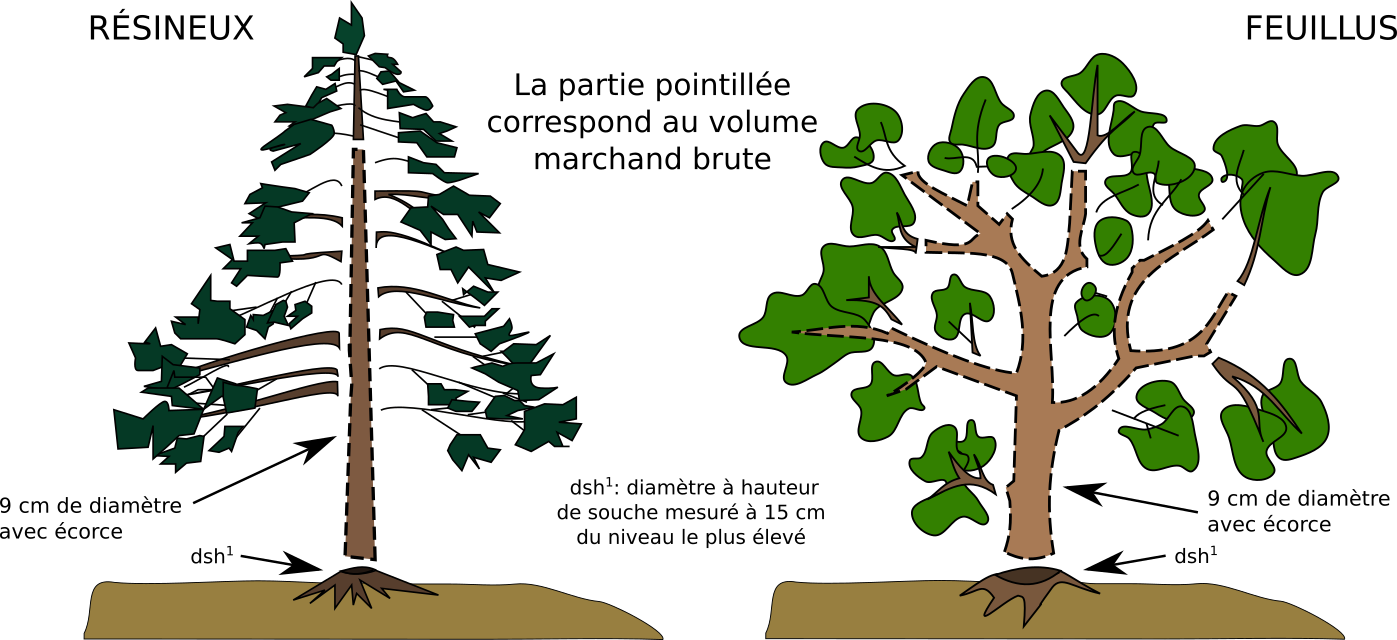
\includegraphics[scale=0.7]{img/ch2_volume_marchand}
\caption{Volume marchand brut (adaptée de \cite{quebec2003tarif} par Joëlle Berthier}
\label{volume_march}
\end{figure}

\subsection{La tige en plan transversal (RT)}

\subsubsection{Cernes annuels}
 
On peut distinguer les cernes annuels suite à la variation du diamètre des cellules et de l'épaisseur des parois cellulaires au cours de la saison de croissance. On distingue le bois initial (aussi appelé bois de printemps) produit au début de la saison de croissance et le bois final (aussi appelé bois d'été) produit à la fin de la saison de croissance (Figure~\ref{josza}). On peut mettre en évidence les caractéristiques suivantes: 

\begin{itemize}
\item Le diamètre des cellules est plus grand et les parois cellulaires plus minces dans le bois initial; 
\item Chez les résineux, la transition du bois initial au bois final peut être graduelle ou abrupte. Chez les feuillus à zone poreuse, elle est abrupte alors que les cernes annuels peuvent être difficiles à distinguer chez certains feuillus à pores diffus; 
\item Le bois final est généralement produit lorsque la croissance en hauteur de l'arbre est ralentie ou complétée; 
\item La masse volumique est plus faible dans le bois initial; 
\item Le bois final est de couleur plus foncée; 
\item La largeur des cernes annuels varie en fonction des espèces, des arbres d'une même espèce, des conditions de croissance, de la hauteur dans l'arbre et des caractéristiques de la cime (hauteur de la cime vivante, nombre de branches); 
\item Des cernes annuels anormaux dits \og cernes discontinus \fg ne font pas le tour de la tige. C'est un cas d'exception que l'on retrouve surtout chez les arbres surannés ou dominés. Le bois obtenu de ces arbres est de mauvaise qualité; 
\item Les \og faux cernes \fg sont des cernes continus à l'intérieur d'un cerne annuel \og normal \fg. Ils peuvent être causés par une défoliation, une sécheresse ou des conditions favorables en fin de saison de croissance.  
\end{itemize}
 
\begin{figure}[h]
\centering
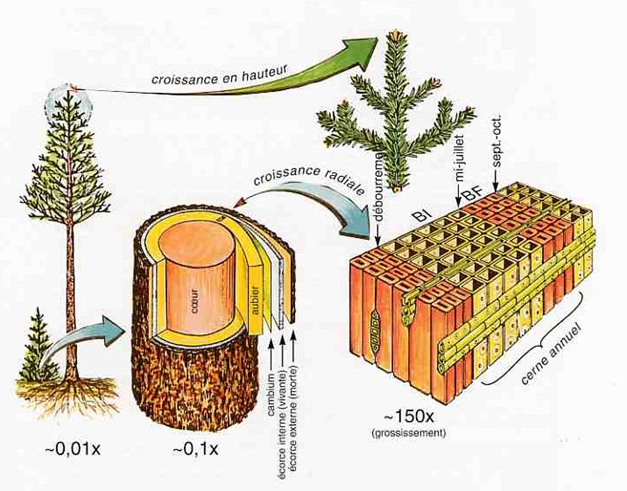
\includegraphics[width=\textwidth]{img/ch2_josza}
\caption{Facteurs régissant la croissance de l'arbre et la production de bois initial et de bois final dans les cernes annuels (image tirée de \cite{jozsa1994discussion})}
\label{josza}
\end{figure}

\subsubsection{Bois d'aubier et bois de duramen}
 
Chez de très jeunes arbres, toute la section de la tige est utilisée pour la conduction de la sève brute et l'entreposage des substances nutritives. Ce bois est appelé bois d'aubier. Les ponctuations ouvertes que l'on rencontre dans les cellules du bois d'aubier permettent le passage de la sève brute. Les cellules de parenchyme sont vivantes et utilisées pour l'entreposage. À mesure que l'âge cambial augmente, la section complète n'est plus nécessaire et les cellules de la partie centrale de la tige cessent de fonctionner. Le bois de duramen est alors formé. Les parenchymes meurent et les cellules axiales perdent leurs propriétés de conduction des liquides. Des substances extractibles se déposent dans les parois cellulaires et donnent au duramen sa couleur généralement plus foncée.\\

On peut mettre en évidence les caractéristiques suivantes pour le bois d'aubier et le bois de duramen: 

\begin{itemize}

\item Aubier
	\begin{itemize}
	\item Support mécanique de la tige; 
	\item Transport de la sève; 
	\item Entreposage des substances nutritives dans les parenchymes vivants. 
	\end{itemize}

\item Duramen
	\begin{itemize}
	\item Les parenchymes meurent; 
	\item Les cellules axiales deviennent moins perméables et n'assurent plus qu'un rôle de support mécanique; 
	\item Il y a formation d'extractibles causant un changement de couleur du bois plus ou moins important; 
	\item Certaines espèces (ex. bouleau blanc, hêtre) ne forment pas de \og vrai \fg duramen mais plutôt du bois coloré d'origine traumatique dont le développement est initié par des blessures ou autres traumatismes subis par l'arbre sur pied. Pour la transformation du bois, c'est souvent la couleur qui importe plus que les processus physiologiques.  
	\end{itemize}
 
\item Aubier \og coloré \fg
	\begin{itemize}
	\item Zone intermédiaire entre l'aubier et le duramen; 
	\item Présence de parenchymes vivants; 
	\item La coloration est présente;
	\end{itemize} 
\item Perméabilité
	\begin{itemize}
	\item La perméabilité du bois de duramen est généralement inférieure à celle du bois d'aubier; 
	\item Présence de substances extractibles bloquant les ponctuations; 
	\item Tyloses chez certains feuillus (ex.: chêne blanc); 
	\item Aspiration des ponctuations aréolées chez les résineux.
	\end{itemize} 
 
\item Résistance à la pourriture
	\begin{itemize}
	\item Le bois de duramen est généralement plus résistant aux champignons de pourriture à cause de la présence des substances extractibles. 
	\end{itemize} 
 
\item Teneur en humidité
	\begin{itemize}
	\item Tel que présenté au Tableau~\ref{humidite}, la teneur en humidité du bois d'aubier des résineux est beaucoup plus élevée que celle du bois de duramen alors que chez les feuillus, il n'y a pas de différences significatives.
	\end{itemize} 
	
\item Largeur du bois d'aubier dépend de:
	\begin{itemize} 
	\item Espèce 
	\item Arbres 
	\item Hauteur 
	\end{itemize}
% 
\item Couleur du bois
	\begin{itemize}
	\item La couleur du bois est surtout due aux substances extractibles; 
	\item La couleur plus foncée du bois de duramen est recherchée chez certaines espèces exemples: chênes, noyers, acajous, cerisier tardif. 
	\end{itemize}
\item Odeur du bois
	\begin{itemize}
	\item L'odeur du bois est causée par les substances extractibles dans le duramen et la présence de champignons et de bactéries. Par exemple, l'odeur forte du genévrier rouge \textit{(Juniperus virginiana)} est due aux extractibles du bois de duramen.
	\end{itemize}

\end{itemize} 

\begin{table}[ht]

\centering
	
	\begin{tabular}{l c c}
	\hline
	\bf Espèce	& \bf Aubier & \bf Duramen \\
	\hline\hline
	Épinette blanche  & 144 &  38\\
	Épinette noire   & 113 & 52 \\
	Pin blanc   & 175 &  50 \\
	Sapin baumier   & 173  & 88 \\
	Thuya occidental  & 240 &  32 \\
	\hline
	Érable à sucre   & 72 &  65 \\
	Bouleau jaune   & 68 & 70  \\
	Chêne rouge   & 69 &  80 \\
	Frêne blanc   & 44 & 46 \\
	Peuplier faux-tremble  & 113 & 95 \\
	\hline
	\end{tabular}

\caption{\label{humidite} Teneur en humidité (\%) à l'état vert du bois d'aubier et du bois de duramen}
\end{table}
~
\todo{Notez que chez les résineux, la teneur en humidité de l'aubier est beaucoup plus élevée que celle du duramen, alors que ce n'est pas le cas chez les feuillus} 

\subsection{Le grain du bois et la pente du fil}
 
Le grain ou fil du bois désigne l'alignement longitudinal des cellules du bois. On définit alors le bois à fil droit, le bois à fil spiralé et le bois à fil croisé ou contrefil tel qu'illustré à la Figure~\ref{fil}. 


\begin{figure}[h]
\centering
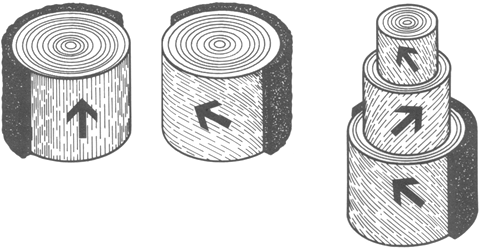
\includegraphics[scale=0.7]{img/ch2_fil}
\caption{Grain ou fil du bois (image tirée de \cite{bowyer2007forest}). De gauche à droite: fil droit, fil spiralé, fil croisé.}
\label{fil}
\end{figure}

\subsection{L'écorce}

L'écorce a pour fonctions principales la protection contre la dessiccation, les blessures mécaniques, les insectes et les maladies. Une représentation schématique de l'écorce est présentée à la Figure~\ref{ecorce}. 

\begin{figure}[h]
\centering


\subfloat[Début de la formation du suber]{%
	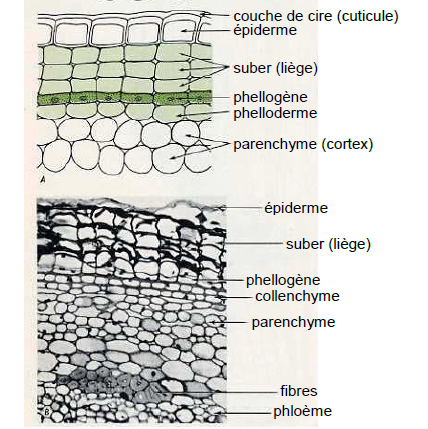
\includegraphics[height=6cm]{img/ch2_coupe_ecorce}
}
~
\subfloat[Représentation schématique]{%
	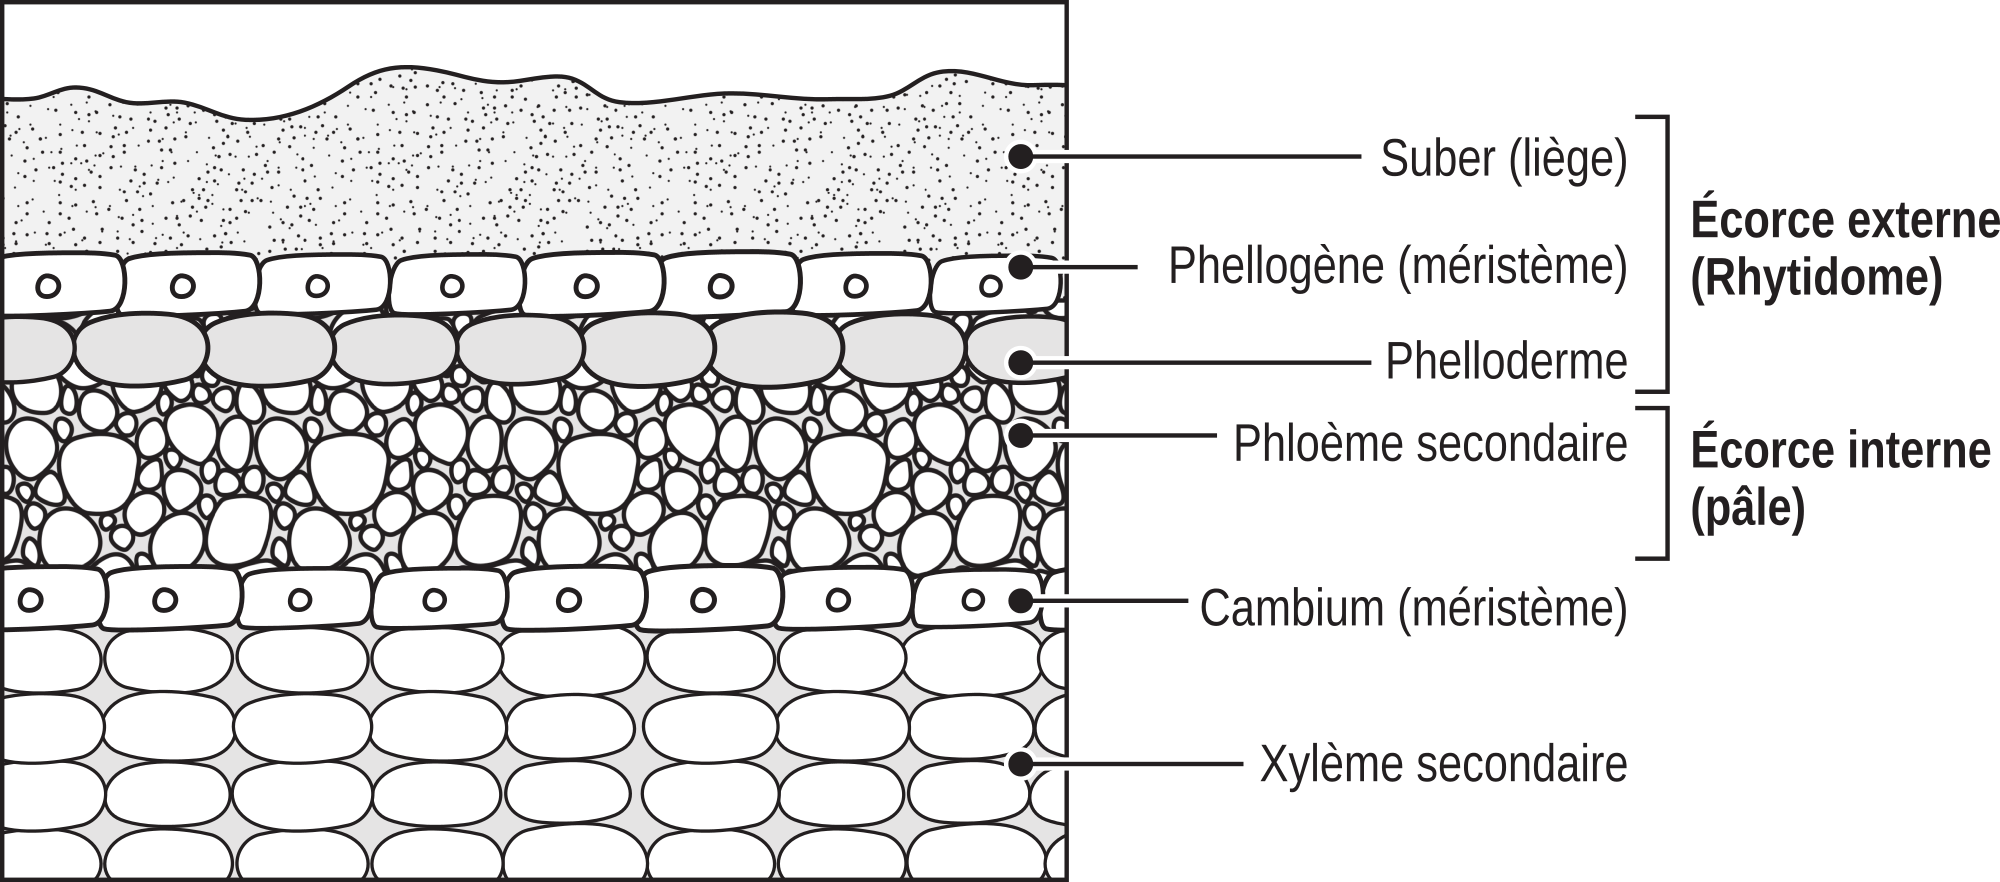
\includegraphics[scale=0.52]{img/ch2_ecorce}
}

\caption{Représentation schématique de l'écorce  a) formation de la première couche de suber chez une jeune tige (adaptée de \cite{weier1974botany}); b) écorce à un âge cambial plus avancé.}
\label{ecorce}
\end{figure}

\subsubsection{Structure de l'écorce}

On désigne habituellement par le mot écorce les tissus qui sont situés à l'extérieur du cambium vasculaire. Le phloème constitue la première couche de tissus de l'écorce que l'on désigne aussi comme écorce interne. Le phloème a pour fonction la conduction de la sève élaborée des méristèmes apicaux vers le bas de l'arbre. Chez les conifères, le phloème ne contient pas de trachéides comme c'est le cas dans le xylème. Il est constitué de parenchymes longitudinaux et de rayon incluant des cellules criblées (cellules allongées non lignifiées contenant le protoplasme et formées de paroi primaire seulement), de fibres de phloème (cellules de soutien allongées à paroi épaisse et lignifiée) et de cellules pierreuses ou sclérites (cellules de soutien à parois secondaires épaisses, lignifiées, sans protoplasme à maturité). Chez les feuillus, le phloème contient des parenchymes longitudinaux et de rayon, incluant des tubes criblés, des cellules compagnes (cellule sœur d'un élément de tube criblé), ainsi que des fibres de phloème.\\ 
 
L'écorce externe est aussi appelée rhytidome ou périderme (couche composée du phelloderme, du phellogène et du suber). Elle constitue une couche plus foncée à l'extérieur de l'écorce. L'écorce externe se développe à partir d'une couche de cellules méristématiques appelée phellogène. Le phellogène produit le suber du côté extérieur de l'arbre et une mince couche de cellules appelée phelloderme vers l'intérieur.  Les parois des cellules du suber contiennent de la subérine, une substance cireuse qui rend le suber imperméable à l'eau et aux gaz. Le même périderme peut fonctionner un nombre variable d'années en fonction des espèces. Pour plusieurs espèces, on pourra distinguer le suber produit à chaque année en forme de cercles concentriques.   

\subsubsection{Utilisations de l'écorce }

\begin{itemize}
\item Bouchons de liège (\textit{Quercus suber}); 
\item Tannins pour cuir: pruches (\textit{Tsuga canadensis}, \textit{Tsuga heterophylla})  châtaignier d'Amérique (\textit{Castanea dentata}) 
\item Combustible; 
\item Composte; 
\item Litière; 
\item Panneaux agglomérés; 
\item Médicaments : L'aspirine est produite à partir de l'acide salicylique extrait de l'écorce de \textit{Salix alba} (maintenant synthétisé). 
\end{itemize}
 
\section{La physiologie de l'arbre}

L'arbre est donc une plante qui se distingue des autres notamment par sa grande taille. Cette caractéristique lui permet d'aller chercher une grande quantité de lumière, ce qui est essentiel à son développement et à sa survie. En revanche, cette caractéristique le soumet à d'importantes contraintes mécaniques induites notamment par le vent. Pour s'assurer de rester sur pied (et en vie) l'arbre doit donc être muni d'une tige (ou tronc) de bon diamètre. L'arbre est donc placé devant un important dilemme : utiliser ses ressources pour aller chercher la lumière et risquer le renversement ou utiliser ses ressources pour croître en diamètre et risquer de se faire dominer et ne plus avoir accès à la lumière.\\  

En réalité, la croissance de l'arbre est une solution qu'il applique pour faire face non seulement à ce dilemme, mais aussi à de nombreux autres. Si on veut résumer simplement ce qui régit le développement des arbres on peut faire référence aux quatre fonctions principales dans lesquelles ils doivent s'investir : 

\begin{enumerate}
\item Produire un appareil photosynthétique (cime) pour capter la lumière; 
\item Produire une tige et des racines de structure pour se supporter mécaniquement; 
\item Produire des racines fines pour aller chercher de l'eau et des éléments nutritifs; 
\item Produire des fleurs, des fruits et des graines pour se reproduire. 
\end{enumerate}

Pour y arriver, l'arbre doit utiliser les ressources limitées qui lui sont fournies par la photosynthèse. Chaque fonction est donc reliée aux autres et la solution \og choisie \fg par les arbres face à un tel dilemme est à la base de la structure des arbres et de l'anatomie du bois. C'est en effet grâce à leur hauteur, leur diamètre et la résistance mécanique de leur tige que l'on peut utiliser leur bois comme matériau utile à la construction, par exemple. Les sections qui suivent décrivent les principaux processus physiologique d'intérêt pour expliquer l'anatomie et la structure du bois. 

\subsection{La feuille}

La feuille est l'organe spécialisé dans la photosynthèse chez les arbres et autres végétaux supérieurs (Figures~\ref{feuille} et~\ref{feuille_coupe}). 

\begin{figure}[h]
\centering
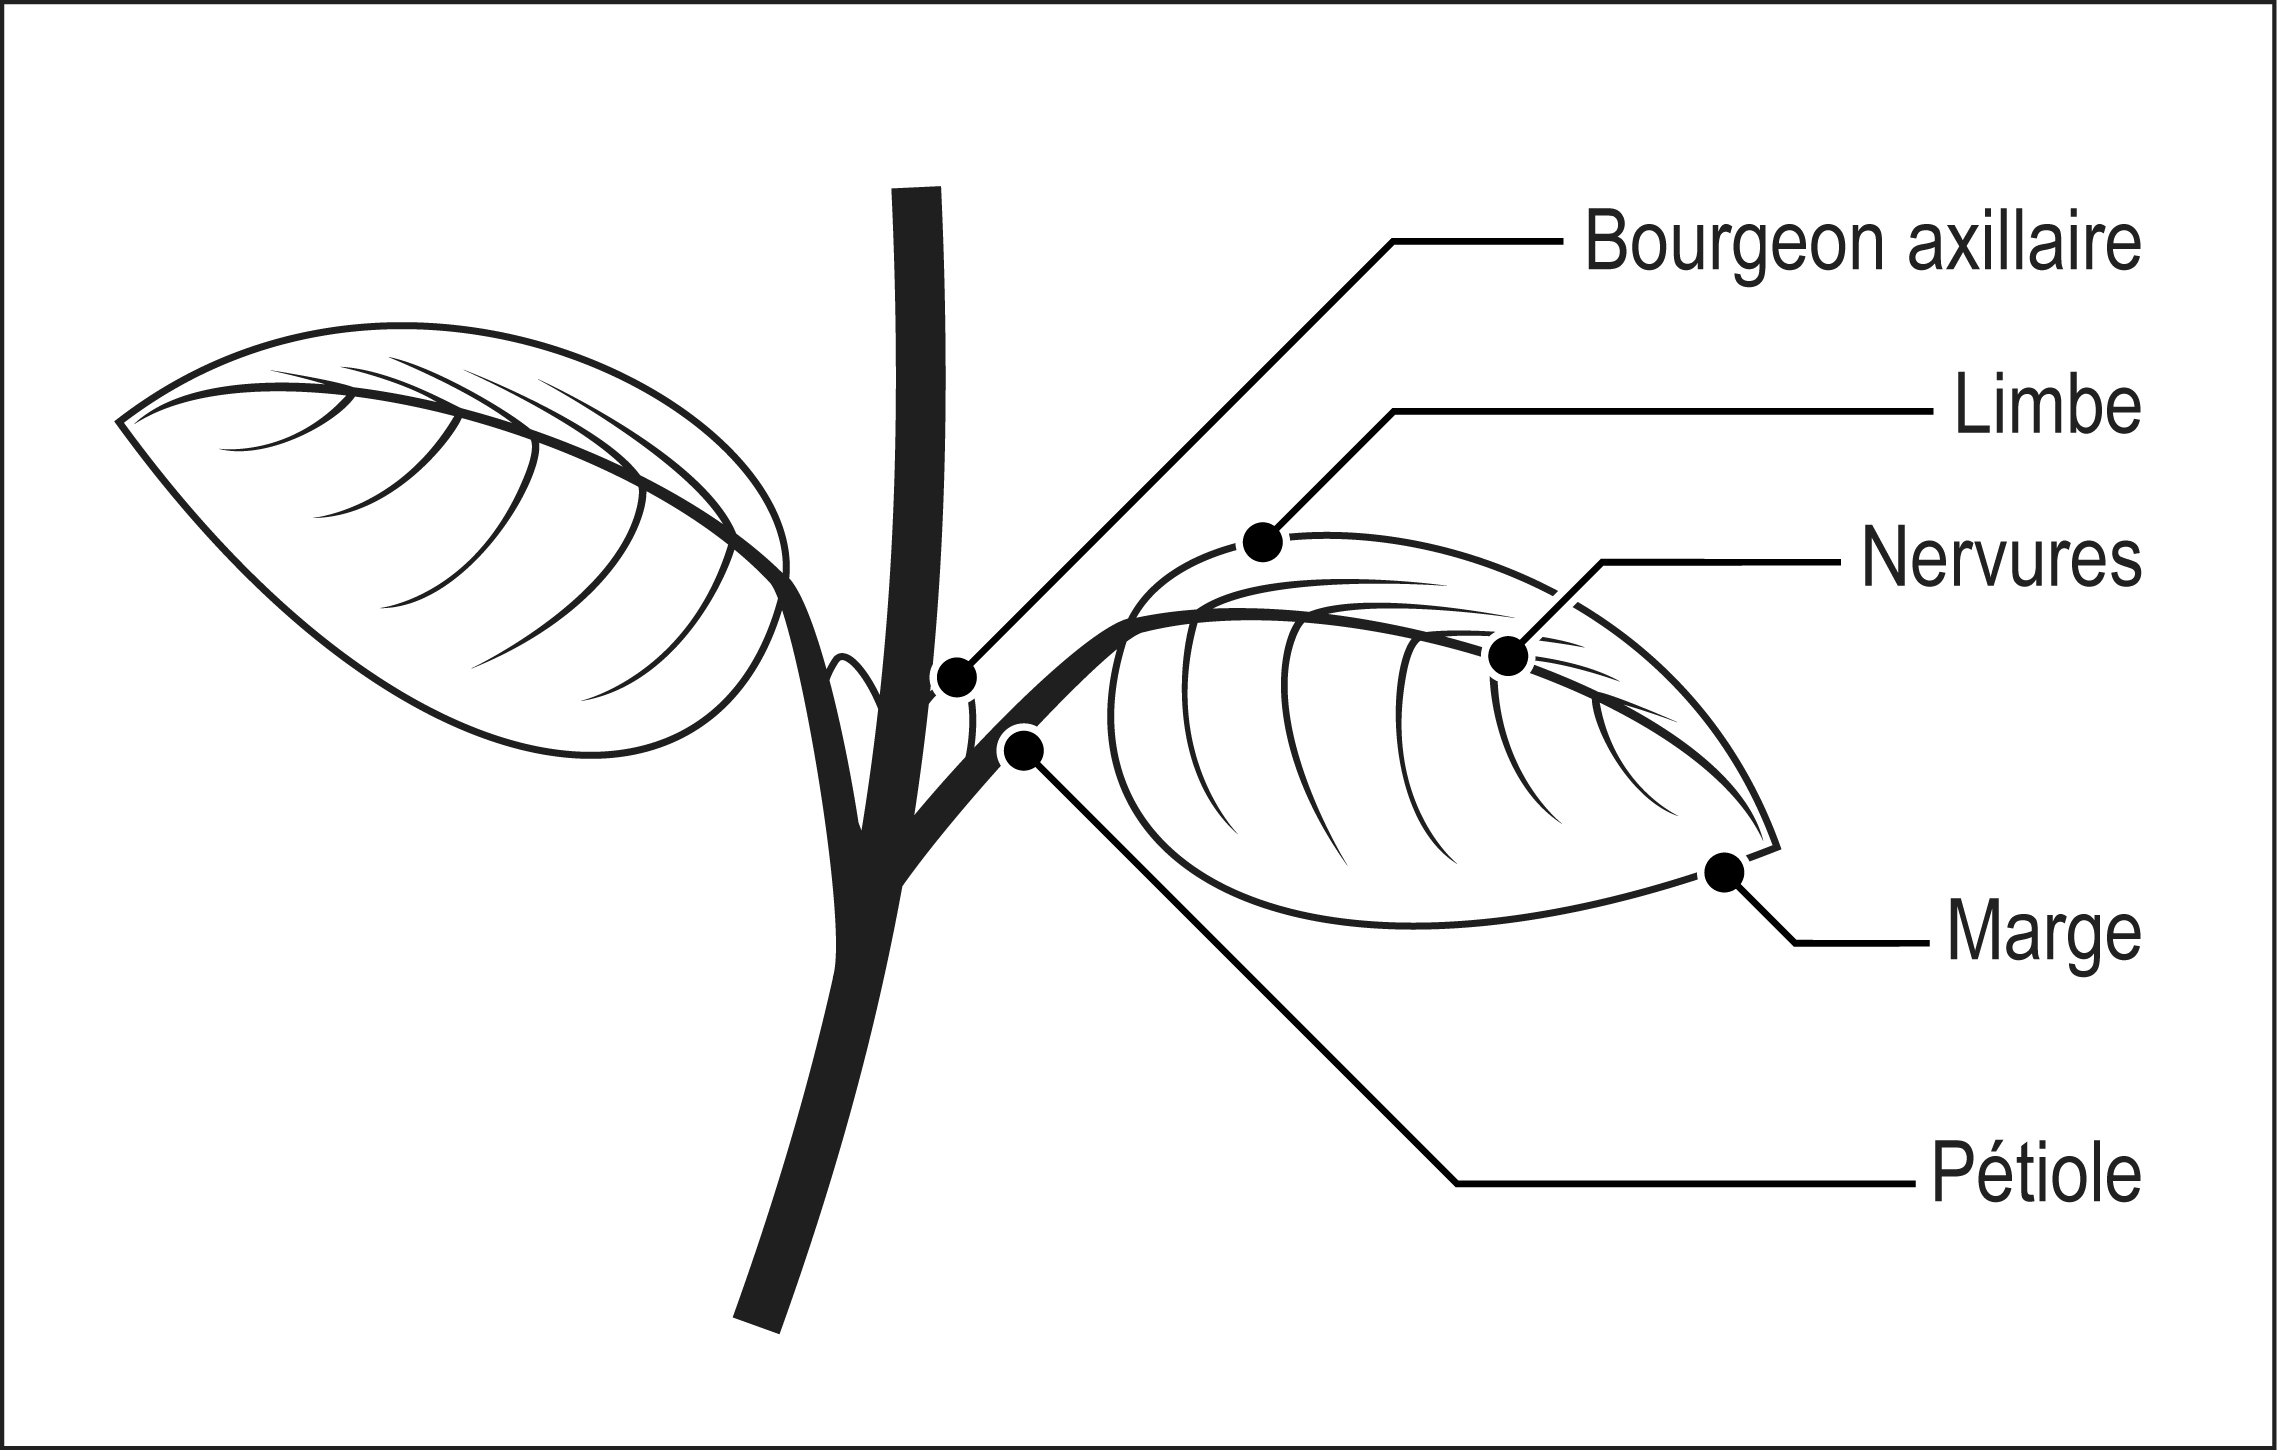
\includegraphics[scale=0.5]{img/ch2_feuille}
\caption{Les parties de la feuille. Image: Julie Ferland }
\label{feuille}
\end{figure}

\begin{description}
\item[Le pétiole] relie le reste de la feuille à la tige (le bourgeon axillaire se situe à la base du pétiole). 
\item[Le limbe] partie souvent plate qui permet à la feuille d'exposer un maximum de surface. 
\item[Les nervures] sillonnent le limbe. Elles sont les prolongements du pétiole et sont donc reliées au reste des tissus conducteurs (xylème – phloème). Le regroupement du xylème et du phloème dans les nervures se nomme faisceau cribro-vaculaire (ou libéro-ligneux) 
\item[L'épiderme] Couche de cellules externes des feuilles couverte par une cuticule (d'aspect cireux)  qui protège la feuille en limitant les pertes en eau.  
\item[Les stomates] Permettent les échanges de O2 et au CO2 avec l'atmosphère. La vapeur d'eau est aussi évacuée par les stomates au cours de la transpiration. Elles peuvent se fermer pour limiter les pertes en eau. 
\item [Le mésophylle] Contient deux types de parenchymes: 
\begin{itemize}
\item Le parenchyme pallissadique (face supérieure) est composé de cellules riches en chloroplastes. Il est responsable de la photosynthèse ; 
\item Le parenchyme lacuneux (face inférieure) est composé de cellules de forme plus arrondie. Les lacunes entre les cellules servent à stocker les gaz échangés entre la feuille et l'atmosphère.
\end{itemize}
 
\end{description}

\begin{figure}[h]
\centering
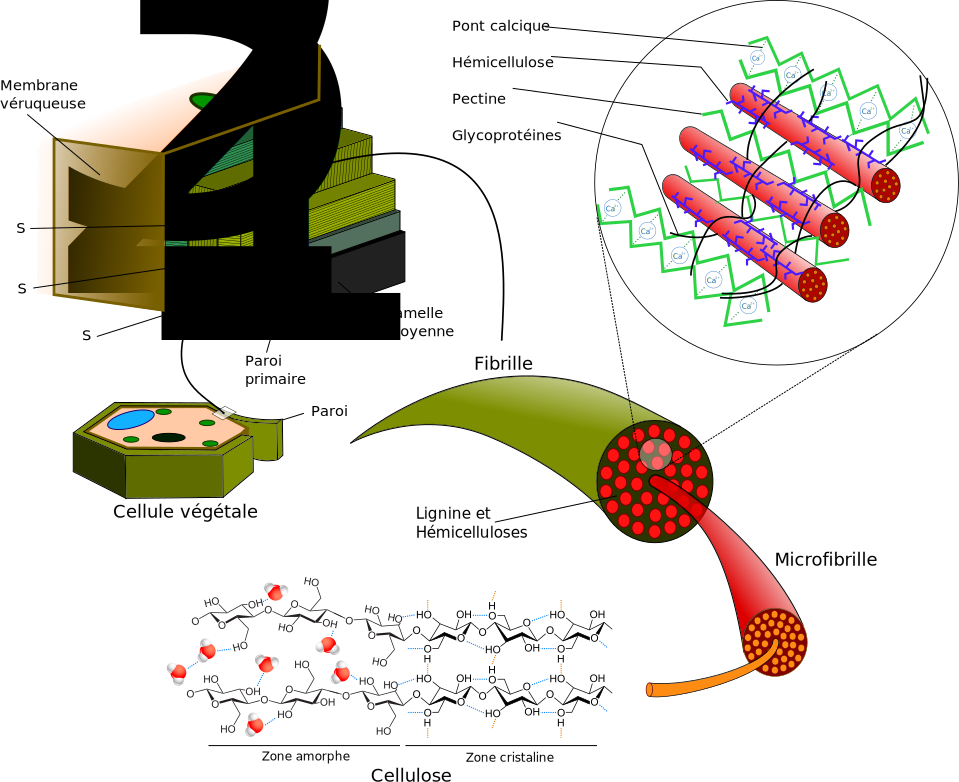
\includegraphics[scale=0.5]{img/ch2_feuille_coupe}
\caption{Anatomie microscopique de la feuille. Adapté de \url{https://fr.wikipedia.org/wiki/Feuille} par Julie Ferland}
\label{feuille_coupe}
\end{figure}

\subsection{Photosynthèse} 

La photosynthèse revêt une très grande importance pour l'ensemble du monde vivant puisque c'est le processus par lequel l'énergie lumineuse est captée et transformée en énergie chimique. La réaction générale de la photosynthèse est la suivante: 

\[CO_2 + H_2O \overset{lumière}{\longrightarrow} CH_2O + O_2\]

L'arbre a donc besoin de CO\sub{2}, d'eau et de lumière pour produire la matière organique nécessaire à sa croissance et à l'accomplissement de ses fonctions vitales. Le processus fournit aussi l'O\sub{2} nécessaire à la respiration cellulaire. Il est intéressant de noter que, contrairement à ce que l'on pourrait penser, l'O\sub{2} provient exclusivement de la molécule de H\sub{2}O et non de celle de CO\sub{2}.\\

La photosynthèse des plantes vertes se divise en deux phases distinctes :  
\begin{description}
\item[La phase lumineuse] qui ne se produit que lorsque la plante est en présence de lumière
\item[la phase sombre] qui peut avoir lieu en présence ou en absence de lumière
\end{description}

Lors de la phase lumineuse, les pigments des cellules photosynthétiques absorbent l'énergie lumineuse et la transforment sous forme chimique par l'entremise de deux produits riches en énergie, l'ATP et le NADPH, tout en libérant de l'oxygène (Figure~\ref{photosynthese}). Pendant la phase sombre, l'ATP et le NADPH générés pendant la phase lumineuse sont utilisés pour réduire le CO\sub{2} atmosphérique et ainsi former du glucose (Figure~\ref{photosynthese}). C'est par ce processus qu'un arbre en croissance peur aider à lutter contre les changements climatiques, puisque le CO\sub{2} atmosphérique est considéré comme le plus important gaz relié à l'effet de serre.\\

Le glucose est un sucre à six carbones qui est couramment retrouvé dans les plantes. Il fait partie de la famille des hydrates de carbones, qui regroupent les composés organiques contenant du carbone, de l'hydrogène et de l'oxygène généralement dans une proportion de 1:2:1. Les hydrates de carbone ont une importance considérable pour les plantes, et ce, de diverses façons : 

\begin{itemize}
\item Premièrement, ils représentent une façon d'entreposer l'énergie provenant de la lumière qui est convertie en hydrates de carbone via le processus de la photosynthèse.  
\item Deuxièmement, ils sont des constituants importants des tissus donnant la structure et la rigidité aux plantes.  
\item Troisièmement, ils fournissent le squelette carboné de plusieurs composés organiques dont les plantes sont constituées.  
\end{itemize}

On verra plus loin que le glucose est l'unité de base de la cellulose, soit un des constituants majeurs de la paroi cellulaire. 

\begin{figure}[ht]
\centering
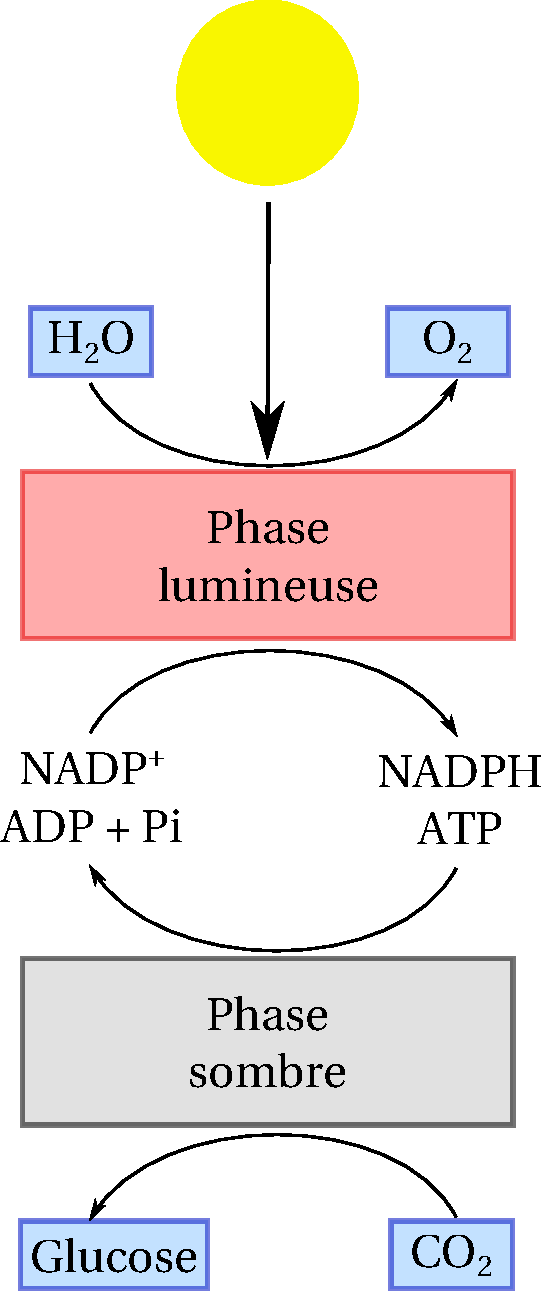
\includegraphics[scale=0.5]{img/ch2_photosynthese}
\caption{Phase lumineuse et phase sombre de la photosynthèse \cite{leninger1993principles}}
\label{photosynthese}
\end{figure}

Quoique le processus de la photosynthèse soit principalement associé à la production d'hydrates de carbone, son mécanisme fondamental consiste à capturer l'énergie lumineuse et de la transformer en énergie chimique à l'aide de pigments sensibles aux longueurs d'onde de la lumière. Ce processus prend place à l'intérieur des cellules végétales vivantes. \\

À une échelle plus fine, une cellule végétale typique possède plusieurs composantes assumant diverses fonctions. Elle est caractérisée par la présence d'une paroi cellulaire et d'une région interne qui est appelée le protoplaste. Le protoplaste est composé du cytoplasme, du noyau, d'une vacuole (qui peut atteindre 95\% du volume de la cellule), et de diverses autres substances comme des tannins, des grains d'amidon, des huiles, etc. Dans le cytoplasme, on retrouve des structures comme des chloroplastes, mitochondries, appareils de Golgi, réticulum endoplasmique, etc. \\

Les phases lumineuse et sombre de la photosynthèse se produisent toutes les deux dans les chloroplastes des cellules qui constituent donc les centrales énergétiques des cellules. La chlorophylle, le pigment donnant la couleur verte aux feuilles des plantes, est le plus important de tous les pigments impliqués dans le processus de la photosynthèse. Plusieurs types de chlorophylle peuvent être distingués, mais les plus abondants sont les chlorophylles a et b qui différencient notamment par leur spectre d'absorption de la lumière. Les chlorophylles a et b ont respectivement des maxima d'absorption dans les régions du orange-rouge et bleu-violet du spectre du visible. Le fait que les deux types de chlorophylle ne montrent que très peu d'absorption dans les longueurs d'onde du vert et du jaune (500 à 600 nm) donne la couleur caractéristique aux feuilles.\\

Plusieurs facteurs interagissent pour influencer la photosynthèse des plantes : 

\subsubsection{La quantité et la qualité de lumière}

Comme on vient de le voir, la qualité de la lumière est fort importante pour le processus de photosynthèse. Par contre, comme la lumière captée par les arbres provient du soleil, il ne s'agit pas d'un facteur facilement modifiable en conditions naturelles.\\

En revanche, la quantité de la lumière est généralement considérée comme un facteur très important pour la croissance des arbres parce qu'elle peut affecter directement le taux de photosynthèse et qu'elle peut être modifiée par des pratiques culturales. Le contrôle de la lumière est le principal outil à la disposition du sylviculteur qui veut influencer la croissance de l'arbre.\\

Les feuilles n'utilisent pour la photosynthèse qu'une petite partie de la lumière incidente. Ainsi, les feuilles sont généralement saturées en lumière à des valeurs inférieures à 50\% de la lumière incidente par temps ensoleillé (Figure~\ref{c_uptake}). 


\begin{figure}[h]
\centering
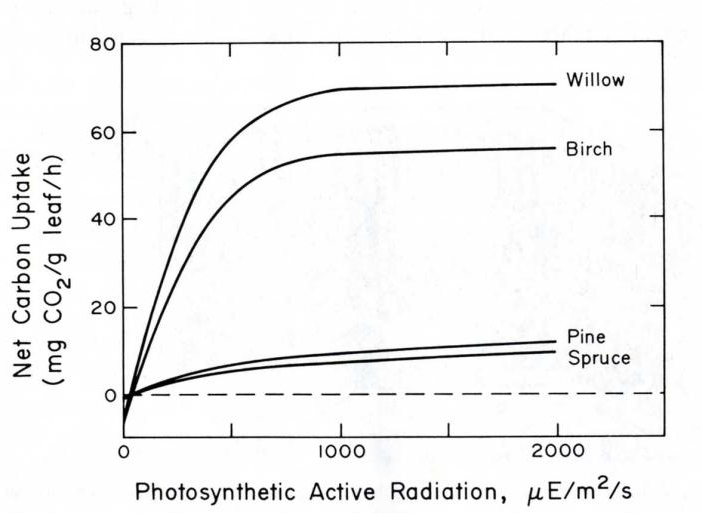
\includegraphics[scale=0.5]{img/ch2_C_uptake}
\caption{Courbe de saturation de la lumière pour différentes espèces forestières \cite{waring1985forest}. }
\label{c_uptake}
\end{figure}	

Cependant, le même phénomène n'est généralement pas observé lorsque toutes les feuilles de la cime d'un arbre sont considérées. En effet, l'ombre créée par les feuilles de la partie supérieure de la cime sur les feuilles du bas de la cime fait en sorte que peu importe l'intensité lumineuse, toutes les feuilles de la cime ne sont pas saturées en même temps. Ainsi, le taux de photosynthèse de la cime d'un arbre continue généralement d'augmenter parallèlement à l'augmentation de l'intensité de la lumière incidente et n'atteint donc pas un plateau comme dans le cas d'une feuille individuelle.\\

Par opposition au concept de saturation de la lumière, il importe aussi de souligner le point de compensation de la lumière de la lumière qui correspond à l'intensité lumineuse à laquelle le CO\sub{2} utilisé pour la photosynthèse est égal à la quantité de CO\sub{2} libéré par la respiration (voir section ~\ref{respiration}). Cette limite varie beaucoup d'une espèce à l'autre. Elle définit la tolérance à l'ombre de celles-ci (tableau~\ref{tolerance}). 

\begin{table}[h]
\centering
	
	\begin{tabular}{l c c}
	\hline
	\bf Espèce	& \bf Point de compensation & \bf Tolérance à l'ombre \\
	\hline
	\hline
	Érable à sucre & 3,4\% & Très tolérant \\
	Pruche de l'est	& 8,4\%	& Très tolérant \\
	Pin blanc &	10,4\% & Intermédiaire \\
	Chêne rouge	& 13,6\% &  Intermédiaire \\
	Pin ponderosa &	30,6\%	& Intolérant \\
	\hline
	\end{tabular}

\caption{Tolérance à l'ombre (d’après \cite{burns1990silvics}) et point de compensation (en~\% de pleine lumière du soleil d’après \cite{kimmins1987forest}) de la pour différence espèces d'Amérique du Nord }
\label{tolerance}
\end{table}

\subsubsection{La température}

Comme tous les processus métaboliques, la photosynthèse a des contraintes liées à la température qui correspondent approximativement à la tolérance des composés protéiniques (environ 0 à 60\textdegree C). D'une façon générale, une augmentation de l'activité photosynthétique est observée parallèlement à une augmentation de la température jusqu'à une température optimale. À des températures plus élevées que cette température optimale, une baisse de l'activité photosynthétique est généralement observée. Bien que le sylviculteur ne puisse avoir un impact direct sur la température régionale, il faut souligner que le contrôle de l'espacement entre les arbres a un impact sur les conditions météorologiques observées dans le couvert forestier. 

\subsubsection{L'eau}

Il est difficile d'établir si un déficit hydrique peut avoir un effet direct sur le taux de photosynthèse. En effet, la quantité réellement nécessaire pour le processus de la photosynthèse est très petite en comparaison à la quantité d'eau nécessaire pour maintenir un arbre en vie. Par conséquent, avant qu'un déficit hydrique puisse affecter directement la photosynthèse, il est très probable que des effets indirects diminuant le taux de photosynthèse se manifesteront avant.\\
 
Les effets indirects d'un déficit hydrique sur le taux de photosynthèse sont provoqués par une diminution de l'hydratation du protoplasme et par la fermeture des stomates de la feuille. À long terme, ces déficits hydriques sont issus d'une faible teneur en eau du sol associée à un faible pouvoir de rétention en eau du sol, de faibles précipitations, etc. Il est cependant à remarquer que des déficits hydriques peuvent aussi survenir à court terme (quotidiennement) lorsqu'une forte demande évaporative de l'atmosphère pendant le jour provoque une fermeture des stomates. 
 
\subsubsection{La quantité de CO\sub{2} et de O\sub{2} }

D'une part, des concentrations élevées de O\sub{2}  dans l'atmosphère peut inhiber la photosynthèse des plantes. Ce phénomène est relié à un taux de respiration plus élevé en présence de lumière.\\

D'autre part, des concentrations élevées de CO\sub{2} dans l'atmosphère augmentent l'activité photosynthétique. Comme dans le cas de la courbe de saturation à la lumière, la courbe de saturation au CO\sub{2}  comporte un point de compensation (au CO\sub{2}  cette fois) correspond à la concentration en CO\sub{2}  pour laquelle le taux de photosynthèse est égal au taux de respiration lorsque l'intensité lumineuse n'est pas limitative. 
 
\subsection{Respiration}\label{respiration}
 
La respiration est en quelque sorte le processus inverse de la photosynthèse. Toutes les cellules actives respirent continuellement, ce qui occasionne une absorption d'oxygène et une libération de CO\sub{2} dans des proportions égales. Même les cellules qui font de la photosynthèse respirent. En effet, elles aussi doivent utiliser l'énergie produite par la respiration pour alimenter leurs processus métaboliques. Une plante qui a dépassé le point de compensation à la lumière a un bilan positif de photosynthèse vs respiration.\\

La respiration est plus qu'un simple échange gazeux. C'est un processus d'oxydoréduction à l'intérieur duquel des composés sont oxydés pour former du CO\sub{2}, et l'oxygène absorbé est réduit pour former du H\sub{2}O. L'amidon, le sucrose et d'autres sucres de même que des lipides, des acides organiques et même des protéines peuvent servir de substrat pour la respiration. L'équation de la respiration dans le cas du glucose par exemple est : 

\[ C_6H_{12}O_6 + 6O_2  \longrightarrow  6CO_2 + 6H_2O + \mbox{énergie} \]

Une partie de l'énergie produite par le processus de la respiration est libérée sous forme de chaleur mais une autre partie est capturée sous forme d'ATP. L'ATP ainsi formé par la respiration peut ensuite être utilisé par la cellule pour ses différents processus métaboliques. 

\subsection{Transport des sucres} 
 
Les cellules vivantes non-photosynthétiques d'un arbre sont dépendantes des cellules photosynthétiques pour s'approvisionner en combustible organique. Cependant, la distance séparant ces deux types de cellule est parfois très grande. Par conséquent, les arbres ont besoin d'un système de translocation des sucres assez rapide et de dimension telle qu'il puisse répondre aux besoins métaboliques des cellules. Ce transport des sucres est assuré par les tubes criblés qui sont des cellules spécialisées du phloème. Ces cellules forment un réseau vasculaire pouvant transporter les sucres synthétisés par les feuilles à toutes les cellules.\\

En plus des hydrates de carbone, des composés azotés (acides aminés, amides et protéines) peuvent se retrouver dans la sève élaborée. Ces substances proviennent des feuilles ou des fruits en état de sénescence et empruntent la voie du phloème pour être relocalisées dans les tissus plus jeunes de la plante. Parmi les autres substances qu'il est aussi possible de retrouver dans la sève élaborée, il y a l'ATP, des enzymes, des ions organiques, des vitamines, des phytohormones, des herbicides, des virus, des spores de champignon, etc.\\

La direction du transport de la sève élaborée peut être latérale ou axiale. Les mouvements radiaux de la sève élaborée se font surtout vers l'extérieur lorsqu'il y a une blessure à l'écorce qui nécessite la formation d'un cal. Toutefois, des mouvements radiaux vers l'intérieur sont aussi rencontrés dans le parenchyme de rayon et ont pour but d'entreposer des sucres dans le parenchyme du xylème.\\

Par ailleurs, des études ont démontré qu'il n'y a que très peu de transport de la sève élaborée en direction tangentielle. Par exemple, une expérience a déjà démontré qu'une défoliation d'un seul côté d'un arbre aura pour effet de diminuer la croissance radiale seulement du côté où les feuilles ont été enlevées, ce qui implique que les feuilles restantes n'alimentent pas le cambium du côté défolié. Dans l'ensemble, les mouvements latéraux sont quantitativement mineurs comparativement au transport axial, i.e. du haut vers le bas ou du bas vers le haut d'un arbre.\\

Le mouvement axial de la sève élaboré n'est pas polaire, i.e. qu'il peut se produire vers le bas et vers le haut d'un arbre Figure~\ref{pomme}. 


\begin{figure}[h]
\centering
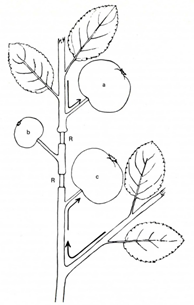
\includegraphics[scale=0.5]{img/ch2_dir_phloeme}
\caption{La croissance de pommes sur une branche annelée à deux endroits \citep{zimmerman1971trees} }
\label{pomme}
\end{figure}

Sur la Figure~\ref{pomme}, une branche de pommier a été annelée à deux endroits, ce qui a eu pour effet d'isoler la pomme b. Si le transport des sucres se faisait uniquement vers le bas de la tige, la pomme c n'aurait pas été approvisionnée en sucres, ce qui aurait diminué sa croissance. À l'inverse, si le transport des sucres se faisait uniquement vers le haut, la pomme a n'aurait pas été approvisionnée en sucres et sa croissance aurait aussi été diminuée. Puisque la croissance des pommes a et c n'a pas été réduite, il faut conclure que le transport de la sève élaborée se fait dans les deux directions.\\

La faible croissance de la pomme b prouve par ailleurs que le transport des sucres se fait bel et bien par le phloème.\\

Non seulement le mouvement axial de la sève élaborée peut se faire dans les deux directions, mais il peut se faire simultanément dans les deux directions. La Figure~\ref{phloeme} illustre ce mouvement bidirectionnel qui implique que les sucres provenant des feuilles peuvent prendre la direction des racines ou ils peuvent être mobilisés vers d'autres points de croissance comme les fleurs, les jeunes feuilles pas encore photosynthétiquement autosuffisantes, ou les fruits. 

\begin{figure}[ht]
\centering
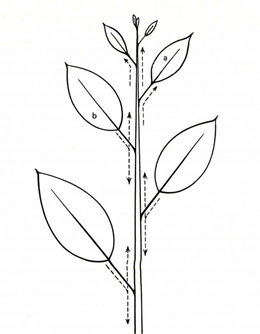
\includegraphics[scale=0.5]{img/ch2_dir_phloeme2}
\caption{Le transport bidirectionnel de la sève élaborée \citep{zimmerman1971trees}}
\label{phloeme}
\end{figure}

D'une façon générale, il a été observé que les feuilles les plus rapprochées des racines (bas de la cime) vont principalement exporter leurs sucres vers les racines (transport vers le bas) alors que les feuilles situées près du sommet de la cime vont principalement exporter leurs sucres vers le haut. Les sucres des feuilles dans une situation intermédiaire seront transportés dans les deux directions.\\ 

À partir d'expériences avec des isotopes radioactifs, il a été possible d'évaluer que la vitesse de transport de la sève élaborée dans le phloème se situait entre 10 et 100 cm/heure, ce qui est remarquablement grand en considérant la taille relativement petite du complexe de tubes criblés qui compose le phloème. Plusieurs hypothèses ont été élaborées pour tenter d'expliquer le mécanisme de transport dans le phloème, mais personne n'a jusqu'ici prouvé qu'une de ces théories était hors de tous doutes le véritable mécanisme. L'étude de ces théories dépasse le cadre de ce cours.\\

\subsection{Transport de l'eau}\label{eau}

Le transport de l'eau brute prend place dans le xylème de l'arbre, ce qui implique qu'il a un important impact sur l'utilisation et la transformation du bois. Physiologiquement, l'aubier représente la partie du xylème qui sert au transport de l'eau (et à l'entreposage des sucres). Tel que présenté au tableau~\ref{humidite}, cette partie de l'arbre a une teneur en humidité beaucoup plus élevée puisque le lumen de ses cellules contiennent de l'eau.\\ 

La force permettant à l'eau de se déplacer du sol jusqu'au sommet d'un arbre est fournie par le gradient de potentiel hydrique entre le sol et l'atmosphère. Puisque l'eau se déplace d'un endroit à fort potentiel vers un endroit à faible potentiel, il faut donc que le potentiel hydrique de l'atmosphère soit plus bas que celui du sol. Cette condition est généralement remplie parce que sous des conditions normales d'humidité relative de l'atmosphère, l'air a un potentiel hydrique beaucoup plus bas que celui du sol. \\

Le faible potentiel hydrique de l'atmosphère généralement rencontré en condition normale fait en sorte que l'eau des feuilles est attirée vers l'atmosphère, et l'évaporation de l'eau qui survient alors à la surface des feuilles est appelé transpiration. À cause de ce phénomène de transpiration, la teneur en eau des cellules foliaires est diminuée, ce qui provoque une baisse de leur potentiel hydrique.\\  

Cette baisse du potentiel hydrique des feuilles aura pour conséquence d'établir un gradient de potentiel hydrique entre les feuilles et le xylème des branches, ce qui aura pour résultat de créer un mouvement d'eau des branches jusqu'aux feuilles.\\ 

En peu de temps, le gradient de potentiel hydrique s'établira partout dans la plante (des feuilles aux racines) et s'étendra finalement jusqu'au sol entourant les racines pour permettre l'entrée de l'eau du sol dans les racines. Ainsi, le gradient de potentiel hydrique qui s'établit entre le sol et l'atmosphère permet aux arbres de puiser l'eau dans le sol et de la retourner dans l'atmosphère par l'entremise de leurs feuilles.\\

Les forces d'adhésion et de cohésion de l'eau sont d'autres propriétés conférant à l'eau une très grande importance pour les plantes.\\

À cause de sa nature polaire (charge positive à une extrémité d'une molécule d'eau et charge négative à l'autre extrémité), l'eau est attirée par plusieurs autres substances, comme les protéines et la cellulose, et les imbibe. Cette attraction entre l'eau et d'autres substances est appelée adhésion.\\

Par ailleurs, l'attraction exercée par les molécules d'eau entre elles est appelée cohésion. Cette force de cohésion entre les molécules d'eau est responsable de la grande résistance de l'eau à la tension et fait en sorte qu'une colonne d'eau de petit diamètre (comme dans une trachéide ou un vaisseau) peut résister à l'application de très fortes tensions. C'est donc cette force de cohésion qui permet à l'eau d'être transportée des racines jusqu'aux feuilles d'un arbre.\\

Chez les gymnospermes (arbres résineux), le transport de l'eau est assuré par des trachéides qui ne sont pas ouvertes à leurs deux extrémités comme les éléments de vaisseau mais qui comportent plusieurs ponctuations principalement concentrées aux deux bouts des trachéides. Puisqu'un certain chevauchement existe entre les trachéides, l'eau peut monter jusqu'au sommet d'un arbre en passant d'une trachéide à l'autre via les ponctuations.\\ 

Puisque les trachéides ont un plus petit diamètre que les vaisseaux et ne sont pas ouvertes à leurs deux extrémités, le transport de l'eau rencontre plus de résistance dans le bois de conifères comparativement aux angiospermes (arbres feuillus). Chez les angiospermes, le transport de l'eau se fait plus rapidement chez les espèces ayant du bois à zones poreuses (ex. : chênes, frênes, orme) que celles possédant du bois à pores diffus (ex. : érables, peupliers, bouleaux).\\

Parmi les autres propriétés de l'eau, il est important de noter que l'eau est un solvant pour plusieurs substances et peut donc servir de véhicule aux acides aminés, aux hydrates de carbone de faible poids moléculaire, aux ions (K+, Ca+2, H2PO4, NO3-, etc.) et à de petites molécules sous forme gazeuse comme l'oxygène. Cette propriété de l'eau, conjointement avec sa force de cohésion, permet donc le transport des éléments minéraux des racines jusqu'aux feuilles.\\ 

\subsection{La nutrition minérale}

Bien que la plante soit principalement formée de matière organique (les composés C, H et O forment ensemble 95\% de la masse anhydre d'une plante), elle a également besoin de nombreux éléments inorganiques puisés dans le sol pour accomplir ses différentes fonctions métaboliques. La Figure~\ref{mineraux} montre la forme de la relation entre la croissance d'une plante et sa concentration en éléments minéraux. 

\begin{figure}[h]
\centering
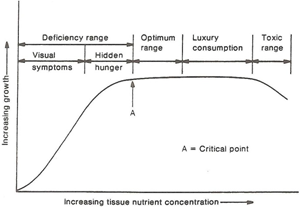
\includegraphics[scale=1]{img/ch2_nutr_min}
\caption{Relation entre la croissance d'une plante et sa concentration en éléments minéraux \citep{landis1989container}}
\label{mineraux}
\end{figure}

En dépit du nombre élevé d'éléments disponibles dans le sol et rencontrés dans les analyses chimiques des plantes, les physiologistes ne reconnaissent actuellement que 16 éléments minéraux indispensables à la croissance de la plupart des plantes. Les éléments essentiels se divisent arbitrairement en deux groupes : les éléments majeurs ou macroéléments qui sont requis en grande quantité (20 à 1000 mg/litre de solution), et les éléments mineurs ou oligoéléments qui sont requis en très petites quantité (<10 mg/litre). La liste de ces éléments est donnée au tableau~\ref{elements}. 

\begin{table}[h]
\centering
	
	\begin{tabular}{l c c}
	\hline
	& \bf Forme d'absorption & \bf Concentration (ppm) \\
	\hline
	\hline
	H & H\sub{2}O &  \numprint{60000} \\
	C &  CO\sub{2}&  \numprint{450000} \\
	O & CO\sub{2}, H\sub{2}O, O\sub{2} & \numprint{450000}  \\
	N &  & \numprint{15000} \\
	K & K\up{+} & \numprint{10000} \\
	Ca & Ca\up{2+} & \numprint{5000} \\
	Mg & Mg\up{2+}  & \numprint{2000} \\
	P &  & \numprint{2000} \\
	S & SO\sub{4} &  \numprint{1000} \\
	\hline
	Cl & Cl\up{-} & 100 \\
	B &  &  20 \\
	Fe &  & 100  \\
	Mn & Mn\up{2+} & 50 \\
	Zn & Zn\up{2+} & 20 \\
	Cu & Mg\up{2+}  & 6 \\
	Mo &  & 0.1 \\
	\hline
	\end{tabular}

\caption{Liste des éléments essentiels à toutes les plantes vasculaires et concentration dans les tissus}
\label{elements}
\end{table}

\subsection{La régulation de la croissance par les hormones}

À partir d'observations et d'expériences, certains chercheurs ont suggéré que des substances chimiques régularisant la croissance étaient présentes dans les plantes. Cette théorie a été proposée pour la première fois par le botaniste allemand Sachs vers la fin du 19e siècle et a été suivie par de nombreuses études qui se poursuivent encore de nos jours.\\

Au fil de ces recherches, une terminologie s'est établie de façon à pouvoir distinguer les substances impliquées dans la régulation de la croissance des végétaux. Ainsi, une phytohormone est définie comme étant un composé organique synthétisé par une certaine partie d'une plante et généralement transporté vers une autre partie de cette plante où, à de très faibles concentrations, il régularise un processus physiologique.\\ 

Cinq groupes de phytohormones jouent des rôles importants dans la physiologie des arbres. Il s'agit des auxines, des gibbérellines, des cytokinines, de l'acide abscissique et de l'éthylène. Parmi celles-ci, les auxines revêtent une importance particulière pour l'anatomie et la structure du bois. 

\subsection{Les auxines}\label{section_auxines} 

Les auxines sont un groupe de substances de structure voisine à l'acide indole 3 acétique (AIA) qui est la plus répandue des auxines naturelles. La découverte des auxines s'est faite en plusieurs étapes. Le premier scientifique qui a contribué à cette découverte fut Darwin qui est mieux connu pour sa théorie de l'évolution que pour ses travaux sur les auxines. Il a démontré que l'inclinaison des tiges et des racines d'une plante en présence d'une source de lumière unidirectionnelle était contrôlée par l'apex. Cette inclinaison des plantes vers la lumière est appelée phototropisme. Darwin a aussi observé que lorsque l'apex de la plante était coupé ou couvert, aucune inclinaison de la plante ne se produisait.\\

Il est possible de retrouver des auxines partout dans une plante mais les plus fortes concentrations se rencontrent dans les apex, les méristèmes et les jeunes feuilles des bourgeons terminaux où ils sont synthétisés. Les plus fortes concentrations d'auxines sont donc rencontrées dans le haut des tiges. En allant vers le bas de la tige, il y a normalement une diminution graduelle de la concentration d'auxines qui est suivie par une augmentation au niveau de la pointe des racines. Un précurseur primaire de l'AIA est le tryptophane qui est un acide aminé. \\

Outre le phototropisme, les auxines régulent plusieurs processus dont notamment la dominance apicale, la production du péricarpe des fruits, l'abscission des feuilles à l'automne, la production racinaire, la formation de cals pour cicatriser les blessures, l'élongation cellulaire et le géotropisme.\\

Les deux derniers éléments de cette énumération montrent que les auxines jouent un rôle primordial pour déterminer les caractéristiques du bois produit par un arbre. La théorie expliquant l'effet de la sylviculture sur la qualité du bois est d'ailleurs centrée sur la concentration de ces hormones dans la plante. Cette théorie, développée par \cite{larson1969wood} sera abordée en détails au chapitre 8.\\

Pour mettre en évidence le lien entre les auxines et la qualité du bois, on peut utiliser le mécanisme par lequel le mode de croissance des plantes est affecté par la force de gravité (le géotropisme). Quand une plante est mise en position horizontale, sa croissance sera déviée de façon à ce que la tige soit dirigée vers le haut (géotropisme négatif) et les racines vers le bas (géotropisme positif). Pour pouvoir orienter sa croissance vers le haut, il faut que la croissance des cellules de la face inférieure de la tige soit plus rapide que celle des cellules de la face supérieure. Cette différence de croissance est possible par une augmentation de la concentration d'auxines dans les cellules de la partie inférieure de la tige qui se ferait à cause de la gravité. On remarque donc qu'une concentration plus élevée d'auxines entraine une activité cambiale plus élevée. \\

C'est par ce même processus que les conditions de croissance affectent le défilement d'une tige. Les arbres croissant en lieux ouverts et n'ayant pas subi d'élagage artificiel ont généralement des branches sur toute la longueur de la tige. À l'opposé, les arbres croissant sous couvert ou ayant subi un élagage artificiel ont moins de branches. Dans un tel cas, la concentration en auxines produites dans les méristèmes apicaux se veut beaucoup plus élevée dans le haut de la tige (tel qu'illustré à la Figure~\ref{auxines}). Comme ces hormones agissent comme démarreur de l'activité cambiale, la croissance en diamètre débute plus rapidement dans la cime vivante au printemps. De plus, la concentration en auxines demeure plus élevée dans la cime vivante tout au long de la saison de croissance, ce qui stimule davantage l'activité cambiale dans cette partie de la tige. Le défilement de la tige est donc moins fort (tige plus cylindrique) pour les arbres possédant une cime vivante moins développée, c'est-à-dire les arbres croissant sur des sites de densité de peuplement plus élevée ou les arbres ayant subi un élagage artificiel. Il est également à remarquer que du bois de type juvénile est produit sous l'effet d'une concentration élevée en auxines, donc dans la cime vivante.  

\begin{figure}[h]
\centering
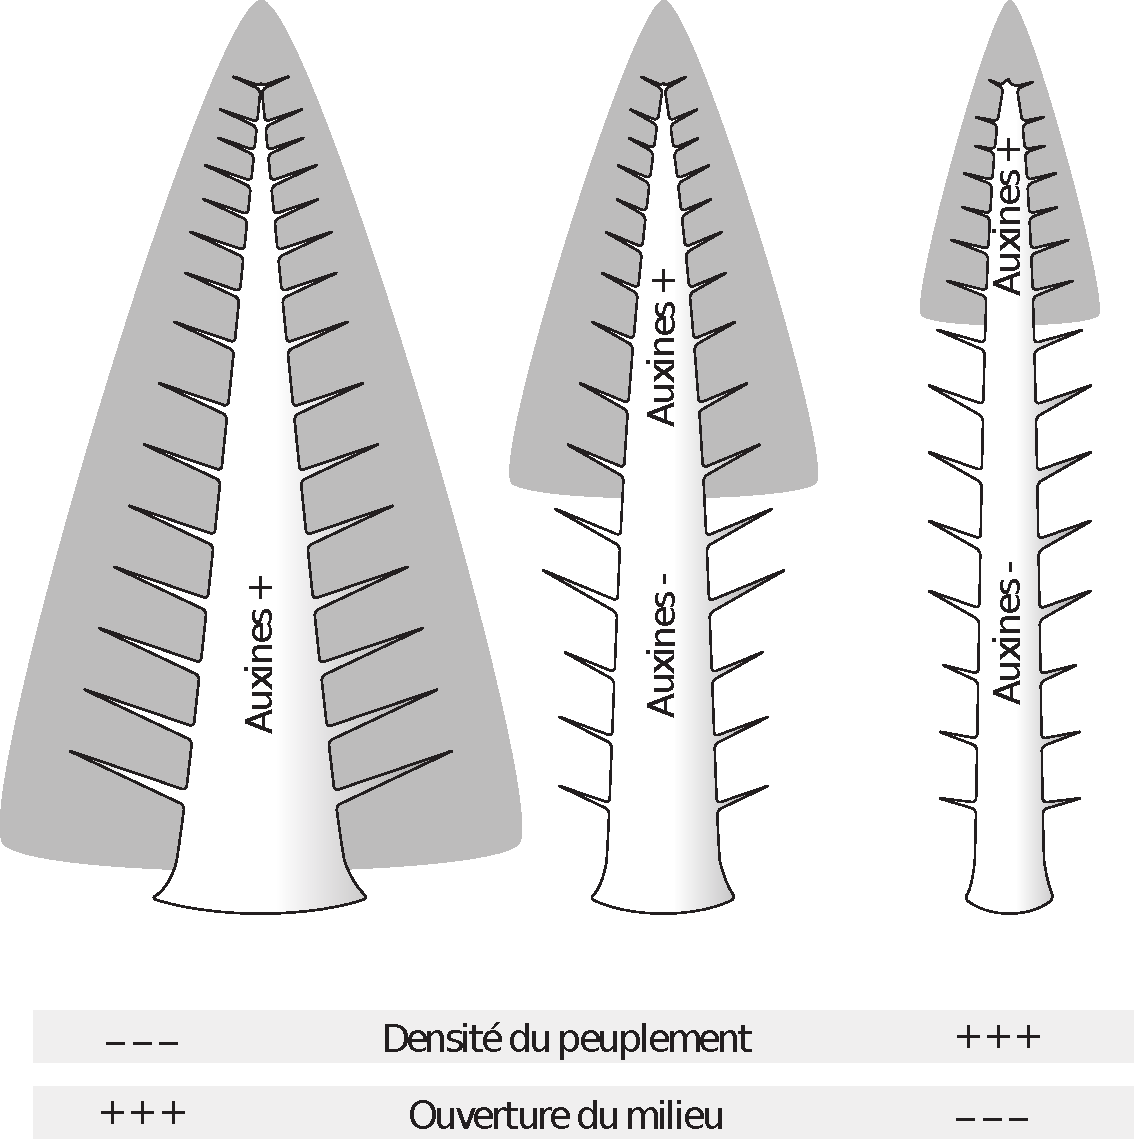
\includegraphics[scale=0.5]{img/ch2_auxine}
\caption{Impact de l'importance de la cime vivante sur le défilement de la tige (adapté de \cite{jozsa1994discussion}. Image préparée par Julie Ferland pour \cite{achim2010dendroecologie}}
\label{auxines}
\end{figure}

% 
%Références 
%Burns, R.M., Honkala, B.H. 1990. Silvics of North America. 654, Vol. 1 Conifers., USDA For. Serv. 675 p. 
%Jozsa, L.A.; Middleton, G.R. 1997. Les caractéristiques determinant la qualité du bois : Nature et conséquences pratiques. Publication spéciale SP-34F, Forintek Canada Corp., Québec. 42 p. 
%Haygreen, J.G.; Bowyer, J.L. 1989. Forest products and wood science. An introduction. Second Edition. Iowa State University Press. Ames, USA. 500 p. 
%Hoadley, R.B. 1990. Identifying wood. Accurate results with simple tools. The Taunton Press Inc. Connecticut, USA. 223 p. 
%Kimmins, J.P. 1987. Forest ecology. Macmillan Publishing Company, New York, U.S.A. 
%Landis, T.D., Tinus, R.W., McDonald, S.E. et Barnett, J.P. 1989. The container tree nursery manual. Volume Four. Seedling nutrition and irrigation. Agric. Handb. 674. USDA For. Serv., Washington, D.C., U.S.A. 
% 
%Larson, P. 1969: Wood formation and the concept of wood quality. Yale Univ. Sch. For. Bull. 74: 1-54. 
%Lehninger, A.L. 1982. Principles of biochemistry. Worth Publishers Inc., New York, U.S.A. 
%MRNF. 2007. Ressources et industries forestières – Édition complète. Ministère des ressources naturelles et de la faune, Gouvernement du Québec. 
%Panshin, A.J.; de Zeeuw, C. 1980. Textbook of wood technology. Fourth edition. McGraw-Hill Book Co. New York. 722 p. 
%Waring, R.H. and Schlesinger, W.H. 1985. Forest ecosystems, concepts and management. Academic Press, London, U.K. 
%Weier, T.E.; Stocking, C.R.; Barbour, M.G. 1974. Botany: An introduction to plant biology. Fifth edition. John Wiley and Sons. New York. 693 p. 
%Zimmermann, M.H. et Brown, C.L. 1971. Trees structure and function. Springer-Verlag, Berlin, Germany. 
% 
% 
